\documentclass[a4paper]{article}
    \usepackage[T1]{fontenc}    %Codifica dei font
    \usepackage[utf8]{inputenc} %Lettere accentate da tastiera
    \usepackage[english]{babel} %Lingua del documento
    \usepackage{tabularx}       % extra features for tabular environment
    \usepackage{booktabs}
    \usepackage[table,xcdraw]{xcolor}
    \usepackage{siunitx}
    \usepackage{fancyvrb}
    \sisetup{output-decimal-marker={,}}
    \usepackage{graphicx} % takes care of graphic including machinery
    \usepackage[margin=0.75in,a4paper]{geometry} % decreases margins
    \usepackage[final]{hyperref} % adds hyper links inside the generated pdf file

    \newcommand{\polito }{\emph{Politecnico di Torino}}
    \newcommand{\oses}{\emph{Operating Systems For Embedded Systems}}

    
    \begin{document}
    \title{
        Projects and Laboratory on Communication Systems - Project Report \\[0.5cm]
        
\includegraphics[width=0.15\textwidth]{PoliLogo.png}%
    }
    \author{Paolo Calao (sxxxxx), Samuele Yves Cerini (s256813), Federico Pozzana (sxxxxx)}

    \date{\today}
    \maketitle
    
    
    \tableofcontents    
    
    \section{The project}

        \subsection{Introduction}
        This final project consists of a Smart-Home Thermostat, realized using \emph{Raspberry Pi3} together with a capacitive touch screen.
        Additional components were added by ourselves in order to positively respond to the given and mandatory requirements.
        While developing the project we have paid particular attention to the organizational phases, trying to think as much as possible as final customers of our product, while delivering something that we hope can be considered something more than a mere \emph{Proof-Of-Concept}.
            
        \subsection{General organization}
        Since the group is composed of 3 people, we divided the project in 3 main components that we will call here, for the sake of simplicity, \textbf{\emph{Backend SW Logic and Web Logic}}, \textbf{\emph{Front-End SW Logic and User Experience}} and finally \textbf{\emph{Hardware and Communication Logic}}.
        Finally, these three main components of the project were merged together during the final phases of the development to build and test the final product.

        \subsection{A Smart-Home Thermostat}
        In this section, we will discuss both mandatory and non-mandatory requirements we implemented for this project, while illustrating our decisions and approaches.
        We intended this Smart-Home Thermostat as a product that targets relatively new buildings, that have been designed with both heating and air conditioning systems.
        Our system is composed by three main Hardware components: the \emph{Central Unit}, composed by a \emph{Raspberry Pi3} and its related capacitive touch-screen, a multiple number of \emph{sensor modules} to retrieve temperature data from each room (built using \emph{ESP32 Microcontrollers}) and finally multiple \emph{actuator modules} that can control the heating system of the building.

        As an example and to keep things in perspective, our home is ideally made of multiple rooms (4 in our case) where each room can be equipped with a stand-alone air conditioner. The heating system for each room is handled by a centralized \emph{actuator module} that groups and drives all the valves required by all the rooms. Each room can have more than one valve serving it, depending on the area to be served by the system, of course.
        Given the aforementioned scenario, our product has been designed to handle more than one room, where each room can be equipped by one \emph{sensor module} (to measure the ambient temperature of the room), as long as an Infrared system to drive a stand-alone air conditioner, if any.

        The \emph{Central Unit} has to be intended as the every-day interface to the system for the customer. It permits to easily add/remove rooms to be controlled, as well as add/remove \emph{sensor modules} and \emph{actuator modules}. We think the system can be easily installed by a normal user with some DIY skills. No big experience is required for using it daily.

        In the following picture we present the main logic organization of the project: we will refer to this image while explaining all the single parts implemented.

        \begin{figure}[htp]
            \centering
            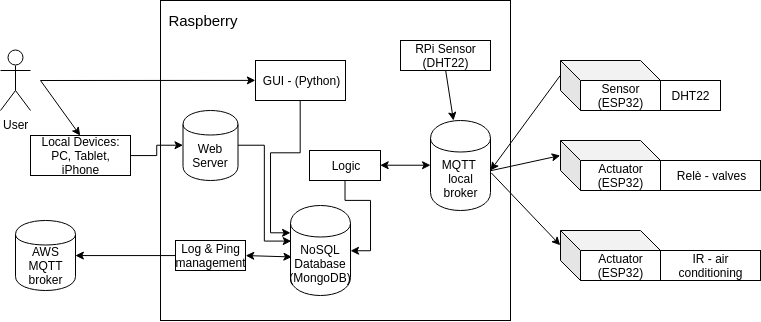
\includegraphics[width=1 \columnwidth]{./Diagram.png}
            \caption{
                    \label{fig:diagram}
                    Logic diagram of the entire project.
            }
        \end{figure}

    \section{Hardware and Communication Logic}

        \subsection{Hardware used}
        The hardware used is the following
        \begin{itemize}
            \item ESP32
            \item relè module
            \item IR receiver and transmitter
            \item thermostatic valve
            \item Li-Ion batteries and relative power supply circuit 
            \item DHT22 temperature sensor
        \end{itemize}
        Here there is a brief explanation for the choice of each component.
        
        \subsubsection{ESP32}
        For this project we needed a processing unit that incorporated both bluetooth and WI-FI functionalities (and possibly with the availability of the relative libraries) ; the choice came down to the ESP8266 and the ESP32. Since they both had the same ease of use in terms of programmability we decided on using the ESP32 because of the much higher pin count. This characteristic made simpler the use of other external components such as the IR transmitter and receiver on the ESP's used as air conditioner remotes and of the relè module on the ESP used as thermostatic valve actuator. 
        
        \subsubsection{Relè module}
        For the ESP used as thermostatic valve actuator we demonstrated the capability of driving a real thermostatic valve with the help of a relè module ; this setup is similar to a real life scenario, where after a command signal the thermostatic valve (driven by the 220V mains voltage) is turned on. The relè module had to be chosen in order to withstand 230V-10A (according to the project specifications). Particular care has been placed into the choice of the relè module for an added specification : since the ESP32 works on 3.3V the module had to be controllable by an high voltage of 3.3V.
        
        \subsubsection{IR receiver and transmitter}
        An added functionality of our project is the capability of firing an IR signal which in a real life scenario would drive the power on and shutdown of an air conditioning system. The IR code can be acquired at the end of the setup of the sensor ESP's, and used as the default code for the air conditioning system. We used a common IR LED for the transmission and a TSOP312x IR receiver for the reception of IR signals. The choice for both the transmitter and receiver were not stringent (most IR transmitters and receivers work on a voltage that spans across 3.3V, our high voltage given by the ESP32) ,however we made sure that there were available libraries to drive these components. With these components we are able to capture ,at the right time during the setup, an incoming IR signal and reproduce it as needed.
        
        \subsubsection{Li-Ion batteries and relative power supply circuit}
        We used Li-ion batteries (18650 form factor) because of two reasons : the large battery capacity (2500 mAh)  and the availability, the batteries ,in fact ,were already available among the group members. To provide a 5V power supply to power up the ESP32 boards we found a circuit specifically made for 18650 batteries that with an input of 3.7V (nominal voltage for a 18650 battery) with a voltage step-up and step-down it provides a stable 3.3V and 5V output.
        
        \subsubsection{DHT22 temperature sensor}
        The choice for the temperature sensor came down to the DHT22 mainly for two reasons; firstly there were the libraries available for the ESP32, and secondly because the project specifications ruled out the DHT11, which was another great option if the project specifications were less stringent.
        
        \subsection{Communication Logic}
        In this section we will highlight the communication protocol used in order to connect the ESP's to the broker running on the RaspberryPy.
        
        \subsubsection{Bluetooth}
        The first communication protocol used is bluetooth; in order to connect either an ESP used as sensor or an ESP used as actuator we establish a bluetooth connection between the ESP and the raspberry, which will send to the ESP some important parameters needed in order to establish a connection between ESP and RaspberryPy broker (these parameters are the network ssid and password and an identifier used during the mqtt connection).
        
        \subsubsection{Wi-Fi}
        The WI-FI communication protocol is used during the mqtt connection between ESP's and broker. During normal use ,in fact, the ESP's used as sensor will send JSON like messages to the broker which ,in turn, will send messages to the ESP's used as actuator in order to configure and drive their capabilities. 
        
        \subsubsection{List of topic used}
        The topic used for every communication can be grouped in four groups
        \begin{itemize}
            \item topic temperatures is the common topic where every sensor publish the current temperature. Particular care has been taken into making the message "readable" by the broker, which has to know which temperature is linked to which room.
            \item topic actuator/configuration is the topic owned by the ESP as an actuator for the thermostatic valves. Its purpose is to link a particular room to a particular relè.
            \item topic actuator/hot/ID ,where ID is the ID of a particular room, is the topic used by the ESP as an actuator for the thermostatic valves in order to switch on or off a particular relè.
            \item topic actuator/cold/ID ,where ID is the ID of the actuator, is the topic used by the ESP as an actuator for the air conditioning system in order to fire the IR code which ,in a real life scenario, will turn on or off an air conditioner.
        \end{itemize}
        
        \subsection{Connecion}
        In this section we will explain the actions performed by both the ESP and the RaspberryPy during the connection of a sensor/actuator to the broker.
        
        \subsubsection{Standard connection}
        During the first connection between the RaspberryPy and any ESP ,regardless of their functionality (sensor/actuator), firstly a bluetooth connection is established : with this connection important parameters such as ssid and password are passed down to the ESP, which will store them for later use. After all the parameters are passed to the ESP the bluetooth connection is killed, and ESP's and RaspberryPy can communicate only via mqtt messages.
        
        \subsubsection{Reset connection}
        Since the parameters used to connect to the broker are stored in the EEPROM of the ESP32, after the first connection an event such as a power failure or hard reset does not cause an indefinite disconnection from the broker, but only a momentary disconnection from it.

    \section{Back-end SW Logic and local Web logic}
    
        \subsubsection{Database}
        In order to save the system's information ,such as configurations, logs etc.., our choice came down to a NOSQL database. The main reason is due to the fact that the information's format that we have to transmit through the broker is the same as the one used by our database, so no further manipulation is needed. The name of our database is MongoDB : MongoDB is a general purpose, document-based, database built for modern application developers and for the cloud era. Furthermore the integration between our system and the database was easy, due to the availability of many resources, such as libraries and guides. In order to connect to the database from the RaspberryPy we used a python software component which includes the following library : PyMongo.
        
        \subsubsection{Web application - server}
        The web server is implemented on the Raspberry so that every device connected to the same network of the Raspberry can easily contact it. The architectural style followed in order to implement the access to the server is Representational State Transfer (REST). The REST architecture is based on HTTP; the functioning is based on a pre-defined URL scheme. According to this technology we mapped every system resource management to a specific HTTP method. To implement it we used PHP in order to have an easy and light server's handling. Apache is the most commonly used Web server on Linux systems, for this reason we decide to adopt it. 
        
        \subsubsection{Web application - client}
        For the front-end of our web application we decided on using a Javascript framework called AngularJS. This framework allowed us to create a single page application on which only the data of interest are fetched continuously, while the main page isn't reloaded. The aim of this application is letting the user interact with the system, such as modifing the configuration and looking at temperatures and graphs in real time. 
        
        \subsubsection{MQTT communication}
        In order of having every component (sensor/actuator) being able to "talk" a mqtt communication has been chosen. We decided to use this protocol because its lightness, ease of configuration and ease of use. Thanks to the dynamic topic management it is ,in fact, possible to connect external devices to the system at any time. In order to implement this communication a broker mqtt ,called Mosquitto, has been chosen. This broker is one of the fastest and lightest broker that can be found online. Lastly, in order to use the broker from the Raspberry side we used the libraries Paho-MQTT, since a lot of examples can be found on the internet. To let every device connected to the same local network could easily find the Raspberry, a multicast DNS has been adopted which can link names to IP addresses without the presence of a DNS server in the same network. Using this technology we bypassed the problem of the raspberry's IP research to the user inside the local network. In fact all the major operating systems ,such as Linux, Mac OS, iOS, Windows, use this approach. The software used by the raspberry to start the MDNS service is Avahi-Daemon. For the ESP32's the ESPmDNS library has been used.

    \section{Front-End SW Logic and User Experience}
        \subsection{Introduction}
        In this section we explain what are the solutions implemented in order to keep the system as simple as possible to the end user. At the same time, we will explore the solutions adopted for the Graphical User Interface. We truly believe that a smart-thermostat should not be overly-complicated or too much fancy: the functionalities have to be the real and most important point.
        Following this idea, the GUI we implemented tries to complete all the functionalities with the minimum number of interactions from the user. As an example, all the functionalities are at maximum of 3 consecutive windows from the principal one. No gestures have been implemented, just single taps to keep the user input as straight as possible. 

        \subsection{GUI framework and languages used}
        Technically speaking, we decided to implement the GUI using the \emph{QT framework} and libraries since the first moment, but due to the limited time available for development, we chose the \emph{PyQT5} version over the original \emph{C++} version. Although \emph{Python3} is not the best language in terms of speed and overall efficiency (due to its interpreted nature and the presence of a garbage collector), we thought that the tradeoff between the speed and the development time was worthing, especially considering that the \emph{Raspberry Pi 3} processor can perfectly handle this type of load. For some textual inputs a virtual keyboard is invoked (the initial choice initially fell on the \emph{QTvirtualkeboard} module thanks to its high integration with the QTframework. Sadly due to the dated \emph{Raspbian} repositories and dependencies, we were not able to install it and so we were obliged to use the \emph{OnBoard} virtual keyboard. This unexpected issue cost us an entire week of development on itself).

        The most of the GUI interfaces have been roughly designed using \emph{QTDesigner} that returns a QML file (\texttt{.ui} extension) that we finally convert to a \texttt{.py} Python script file. Finally, all the finest modifications have been directly made manipulating the \emph{Python} code.
        Structurally speaking, each different window corresponds to a different python class and file. Sometimes some additional and separate files were needed to handle persistence of system-related data.

        \subsection{Main Window interface}
        The Main Window interface (/texttt{MainWindow.py} file) contains all the most useful information for the end user: the actual temperature and the set temperature. The user can also, with just a single tap, enable the \emph{Manual} or \emph{Programmable} mode, as well as a \emph{Antifreeze} mode.
        The former permits to the user to modify the wanted temperature directly by acting on the $+$ and $-$ buttons on the right side of the window. The \emph{Programmable} mode permits to automatically set the desired temperature according to a program the user specified in a previous moment (if the program has not being specified yet, the GUI returns a "void" symbol).
        Finally, the \emph{Antifreeze} mode permits to the end user to set a temperature of 15 Celsius degrees (very useful when the user is on vacation, for example).
        At the bottom of the main window we can find a list containing all the rooms inserted by the user. The "main" room is the so called \emph{default} one: this room cannot be deleted by the user and corresponds to the room where the \emph{Central Unit} is installed (i.e. the \emph{Raspberry Pi}). By tapping on the left and right arrow, the user can scroll through the list: the data shown in the window changes accordingly to the room name displayed by the list.

        \begin{figure}[htp]
            \centering
            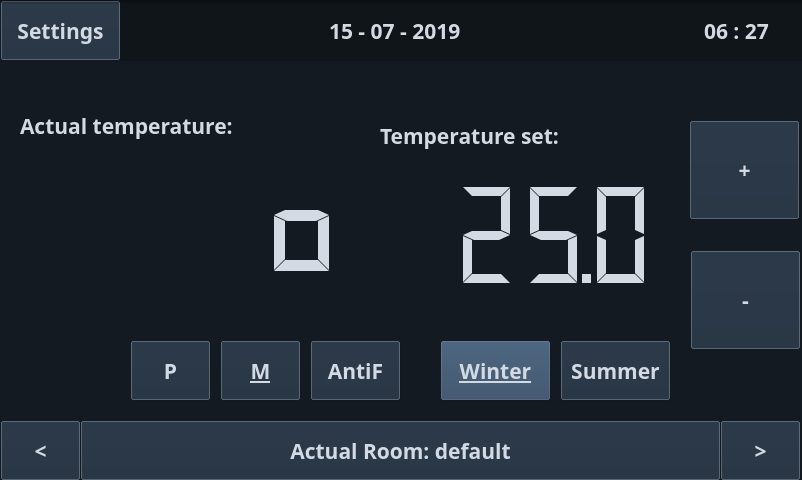
\includegraphics[width=0.8 \columnwidth]{./main.png}
            \caption{
                    \label{fig:main}
                    This is the main window of the system. The LCD on the left indicates the actual temperature retrieved by the sensor, since no sensor was present at the moment of the screenshot, a "void" symbol is displayed.
            }
        \end{figure}

        \subsection{System Settings}
        By tapping on the top-left corner the user can enter the main \emph{System Settings}. Here the user can connect the 
        system to its home WiFi network. The user can also add (or delete) the rooms to be controlled by the system, as long as adding (or deleting) the valve actuators mandatory to handle the heating system of the building.

        \subsection{Local Network connection and related interfaces}
        By tapping on the highest button, the user can enter the \emph{Network Settings Window}. Here it can insert all the credentials of his home WiFi and connect the system to it. This is a crucial step for the entire system, since without connections the system itself loses a big majority of its functionalities.
        The required infos are the \emph{SSID} and \emph{password} of the home network. Since the product is intended like a consumer-grade product, the interface does not ask for additional credentials like certificates etc\dots 
        Under the hood, the connection is handled using the \emph{subprocess} module provided by the \emph{Python} language. This module permits us to leverage the builtin \texttt{BASH}  commands of the \emph{Rasbian OS}, like \texttt{ip, iw, wpa\_supplicant, ping}.
        The system firstly checks for the presence of the SSID: if correct it tries to connect to the network. After some seconds, a \texttt{ping} command is sent to test the wireless connection.
        Finally, this window, when accessed, will notify the user if the connection is still active or not.

        \subsection{Rooms related interfaces}
        Since the system can handle multiple rooms at the same time, the user must be able to logically handle them. To do so, the system is able to let the user add new rooms or delete older ones. The system uses the \emph{MongoDB} database in order to keep the data persistent between reboots of the system.
        A room can have multiple sensors in order to retrieve the ambient temperature. At the same time, an actuator can handle the valves that are connected to the room floor, in order to control the stream of hot water flowing in the pipes.
        Another type of actuator can finally control an AirConditioner, if any.
        Thus, it is mandatory to have a supporting data structure that is both reliable and easy to access. 

        \subsection{Sensors module connection and related interfaces}
        Once the user has added a room into the system, the following step is to connect an actuator to it and link the valves of the heating system to the right actuator. Thus, each room will have a set of valves logically (and finally, physically) connected to the system. Each actuator has a set of 8 relays for a maximum of 8 different valves per actuator. A room, if necessary, can be connected to multiple actuators. Finally, in order to measure the actual temperature, it is necessary to add at least a sensor to the room. The sensor, once connected, will harvest the data regarding the ambient temperature and the send it to the \emph{Central Unit}, that will display it on the guy and, obviously, use it to control the heating and cooling system of the building.
        Following the same approach as before, sensors and actuators can be added/deleted.
        Both sensors and actuators (\emph{ESP32 modules}) are firstly connected via \emph{Bluetooth} to the \emph{Raspberry Pi}. Once the bluetooth connection obtained, all the data necessary for the modules to connect to the home WiFi network is passed and finally an MQTT connection is permanently established.

        \subsection{Program related interfaces}
        As said before, a user has also the ability to set a temperature timetable for each of all the rooms inserted.
        Such schedule will be activated only when the user desires to, by tapping on the \emph{P} button in the main window.
        We decided to keep the schedule as simple and straightforward as possible: since many of us have similar thermostat systems at home, we learnt from our experience that a simpler system that allows a high flexibility gives a overall better user experience.
        We truly believe that a too fine granularity (a hourly one, for example) is often counterproductive and cumbersome for the end user: if too complicated or too long to complete, the user will simply avoid to use it, making it a useless functionality.

        \begin{figure}[htp]
            \centering
            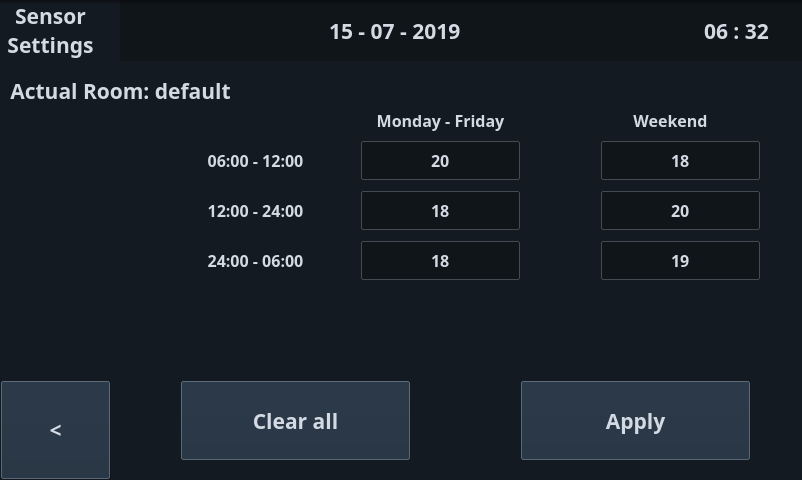
\includegraphics[width=0.8 \columnwidth]{./prog.png}
            \caption{
                    \label{fig:prog}
                    This is the window were the weekly timeschedule is defined. The user can write the temperatures desired to the boxes corresponding to the time slot. The choice is confirmed by tapping on the \emph{Apply} button.
            }
        \end{figure}

 
    \end{document}